\documentclass[a4paper]{article}
\usepackage[utf8]{inputenc}
\usepackage{amsmath}
\usepackage{amssymb}
\usepackage{mathtools}
\usepackage{amsfonts}
\usepackage{lastpage}
\usepackage{tikz}
\usetikzlibrary{patterns}
\usepackage{pdfpages}
\usepackage{gauss}
\usepackage{fancyvrb}
\usepackage[table]{colortbl}
\usepackage{fancyhdr}
\usepackage{graphicx}
\usepackage[margin=2.5 cm]{geometry}
\pagestyle{fancy}
\def\checkmark{\tikz\fill[scale=0.4](0,.35) -- (.25,0) -- (1,.7) -- (.25,.15) -- cycle;} 
\newcommand*\circled[1]{\tikz[baseline=(char.base)]{
            \node[shape=circle,draw,inner sep=2pt] (char) {#1};}}
\newcommand*\squared[1]{%
  \tikz[baseline=(R.base)]\node[draw,rectangle,inner sep=0.5pt](R) {#1};\!}
\cfoot{Page \thepage\ of \pageref{LastPage}}
\DeclareGraphicsExtensions{.pdf,.png,.jpg}
\author{Nikolaj Dybdahl Rathcke (rfq695)}
\title{Anden aflevering \\ Data Analysis}
\lhead{Nikolaj Dybdahl Rathcke (rfq695)}
\chead{Data Analysis}
\rhead{Assignment 1}

\begin{document}
\maketitle
\section*{Question 1}
\subsection*{(1)}
The perceptron update role on round $t$ is defined by
\begin{align}
w^T(t+1)=w^T(t)+y(t)x^T(t)
\end{align}
We want to prove that
\begin{align*}
y(t)w^T(t)x(t)<y(t)w^T(t+1)x(t)
\end{align*}
We can use (1) to expand the right hand side, so we get
\begin{align*}
y(t)w^T(t)x(t)&<y(t)(w^T(t)+y(t)x^T(t))x(t) \\
&=y(t)w^T(t)x(t)+y(t)y(t)x^T(t)x(t)
\end{align*}
subtracting $y(t)w^T(t)x(t)$ from both sides yields
\begin{align*}
0&<y(t)y(t)x^T(t)x(t) \\
&=x^T(t)x(t)
\end{align*}
as $y(t)\in \{-1,1\}$. \\
This holds since the RHS will always be positive.

\subsection*{(2)}
The files \texttt{q1\_2a} and \texttt{q1\_2b} shows how the graphs are generated.\\
Figure 1 shows a situation where $x(t)$ is misclassified by $w(t)$ but is classified correctly by $w(t+1)$. The green line shows $w(t)$, the blue line shows $w(t+1)$ and the red lines are the orthogonals to each of them. In this situation 
$w(t)=\left(
\begin{array}{c}
2\\
0\\
\end{array}
\right)$, $x(t)=\left(
\begin{array}{c}
2\\
1\\
\end{array}
\right)$ and $y=-1$. We can then calculate $y(w^Tx)$:
\begin{align*}
-1\cdot \left((2,0)\left(\begin{array}{c}
1\\
2\\
\end{array}\right)\right)=-2
\end{align*}
As this is less than $0$, it is misclassified. After using the first update rule (1), we have that $w(t+1)=\left(
\begin{array}{c}
1\\
-2\\
\end{array}
\right)$. Calculating $y(w^Tx)$ gives us
\begin{align*}
-1\cdot \left((1,-2)\left(\begin{array}{c}
1\\
2\\
\end{array}\right)\right)=3
\end{align*}
Since this is greater than $0$ it is classified correctly.\\
\\
\begin{figure}
\begin{center}
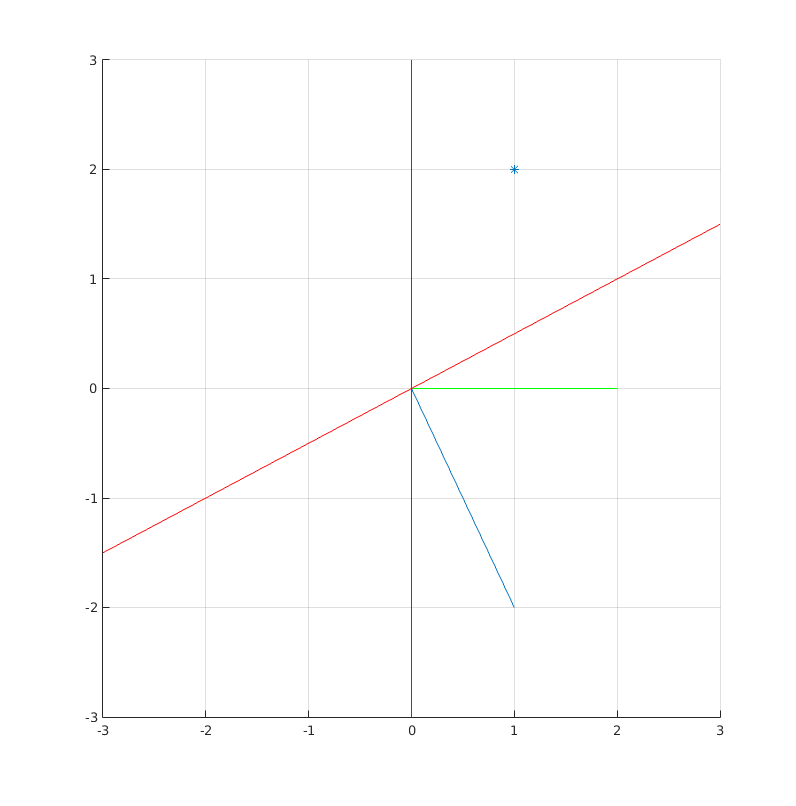
\includegraphics[scale=0.5]{fig1.png}
\end{center}
\caption{$x(t)$ misclassified by $w(t)$ but classified correctly by $w(t+1)$}
\end{figure}
Figure 2 shows a situation where $x(t)$ is misclassified by both $w(t)$ and $w(t+1)$. Again, the green line is $w(t)$, the blue is $w(t+1)$ and the red are the orthogonals. In this situation
$w(t)=\left(
\begin{array}{c}
2\\
2\\
\end{array}
\right)$, $x(t)=(1,2)$ and $y=-1$. Calculating $y(w^Tx)$ yields:
\begin{align*}
-1\cdot \left((2,2)\left(\begin{array}{c}
1\\
2\\
\end{array}\right)\right)=-6
\end{align*}
As this is less than $0$, it is misclassified. After using the first update rule, we have that $w(t+1)=\left(
\begin{array}{c}
1\\
0\\
\end{array}
\right)$. Calculating $y(w^Tx)$ gives us
\begin{align*}
-1\cdot \left((1,0)\left(\begin{array}{c}
1\\
2\\
\end{array}\right)\right)=-1
\end{align*}
This is still less (or equal) than $0$, so it is misclassified. \\
\begin{figure}
\begin{center}
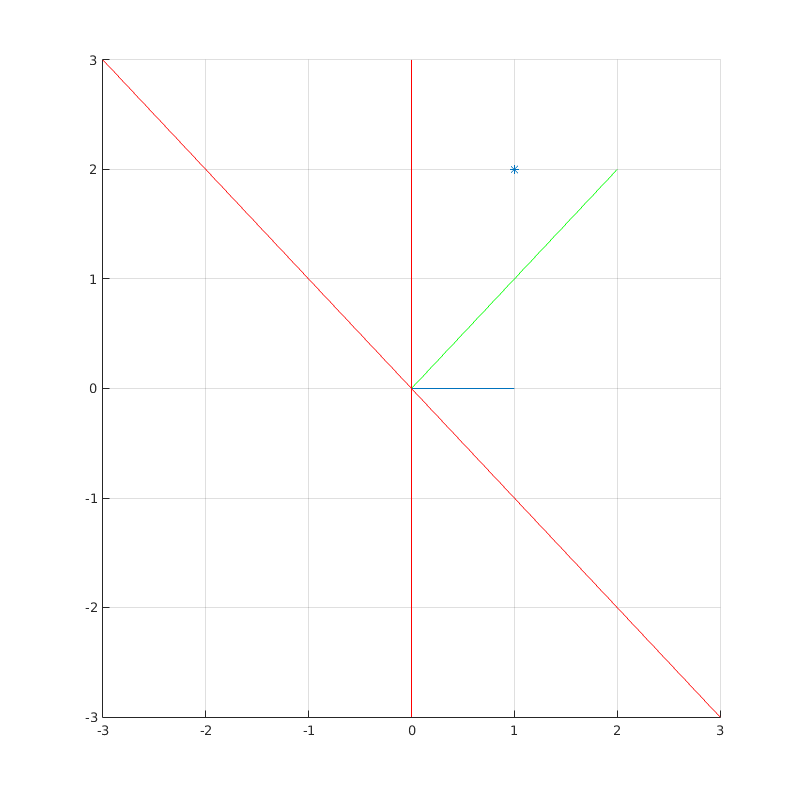
\includegraphics[scale=0.5]{fig2.png}
\end{center}
\caption{$x(t)$ missclassified by both $w(t)$ and $w(t+1)$}
\end{figure}
\\
The rotation is sufficient to classify $x(t)$ when the data is separable by a linear combination through the origin. It is not sufficient if data can only be separated if it is required to rotate around another point.

\subsection*{(3)}
No. The termination condition is that 
\begin{align*}
\exists i \mbox{ s.t. }y_i(w^Tx_i)\leq 0
\end{align*}
When the data is not separable, it means that there will always exists a data point that satisfies this.

\newpage
\section*{Question 2}
\subsection*{(1)}
The linear models uses a signal $s=w^Tx$ that combines the input variables linearly. The perceptron or pocket algorithm are linear classification models, which uses the signal to produce an output which is $\pm 1$ (the sign function).\\
The logistic regression model, though its output is still bounded (it takes values between $0$ and $1$), the produced output is a real number.\\
In our example, when predicting admission, the linear classification model produces a "yes" or "no" answer, while the logistic regression produces a probability that a student is admitted.

\subsection*{(2)}
Running the code to calculate the probability that student $10$ is admitted provides the result $0.4731$.\\
In the file \texttt{q2\_2}, the logistic function $\Theta$ is defined and used with the hypothesis \textit{h}. Running it gives the same result, $0.4731$.

\subsection*{(3)}
The file \texttt{negloglike} implements the function to find the negative log-likelihood, the equation 3.9 [LFD]. \\
Running this from the file \texttt{q2\_3} gives us the following $w$ and $w\_est$ coefficient vectors.
\begin{align*}
w &=
\begin{pmatrix}
   -4.9494 \\
    0.7547 \\
    0.2691
\end{pmatrix}
\\
w_est &=
\begin{pmatrix}
   -4.9494 \\
    0.7547 \\
    0.2691 
\end{pmatrix}
\end{align*}
which are the same.

\subsection*{(4)}
The function is implemented in the file \texttt{errorIn} is based on the equation 3.9 [LFD]. If we use it on $w$, we get $0.6004$.

\subsection*{(5)}
The gradient descent function is implemented in the file \texttt{gradientDesc}. It takes three parameters. The first one, \texttt{init}, is the starting point. The second, \texttt{step}, is the step size $\eta$ and the last one, \texttt{t}, is the number of iterations.\\
It returns two things to make the plot in (7) easy. It returns the last vector $w$, but also a vector for the values of $E_{in}$ for every $500$'th iteration.


\subsection*{(6)}
Using the gradient descent function with parameters \texttt{init}=$[0, 0, 0]$, \texttt{step}=$0.1$ and \texttt{t}=$20000$ provides the result 
\begin{align*}
E_{in}=
\begin{pmatrix}
-4.8774 \\
0.7366 \\
0.2676
\end{pmatrix}
\end{align*}
The result we got from using \texttt{fminunc} was
\begin{align*}
E_{in}=
\begin{pmatrix}
-4.9494 \\
0.7547 \\
0.2691
\end{pmatrix}
\end{align*}
The parameters has been found experimentally, but the two results are close eachother.

\subsection*{(7)}
The relation between iterations and $E_{in}$ is seen in Figure 3 (using $20000$ iterations).\\
The green point is the the value we want to approach. The figure evens out as we get to iteration $t=10000$ and it's close to the green point, so the choice $t=20000$ is an accurate estimate. \\
It has been created with the code from file \texttt{generateFigure}.
\begin{figure}
\begin{center}
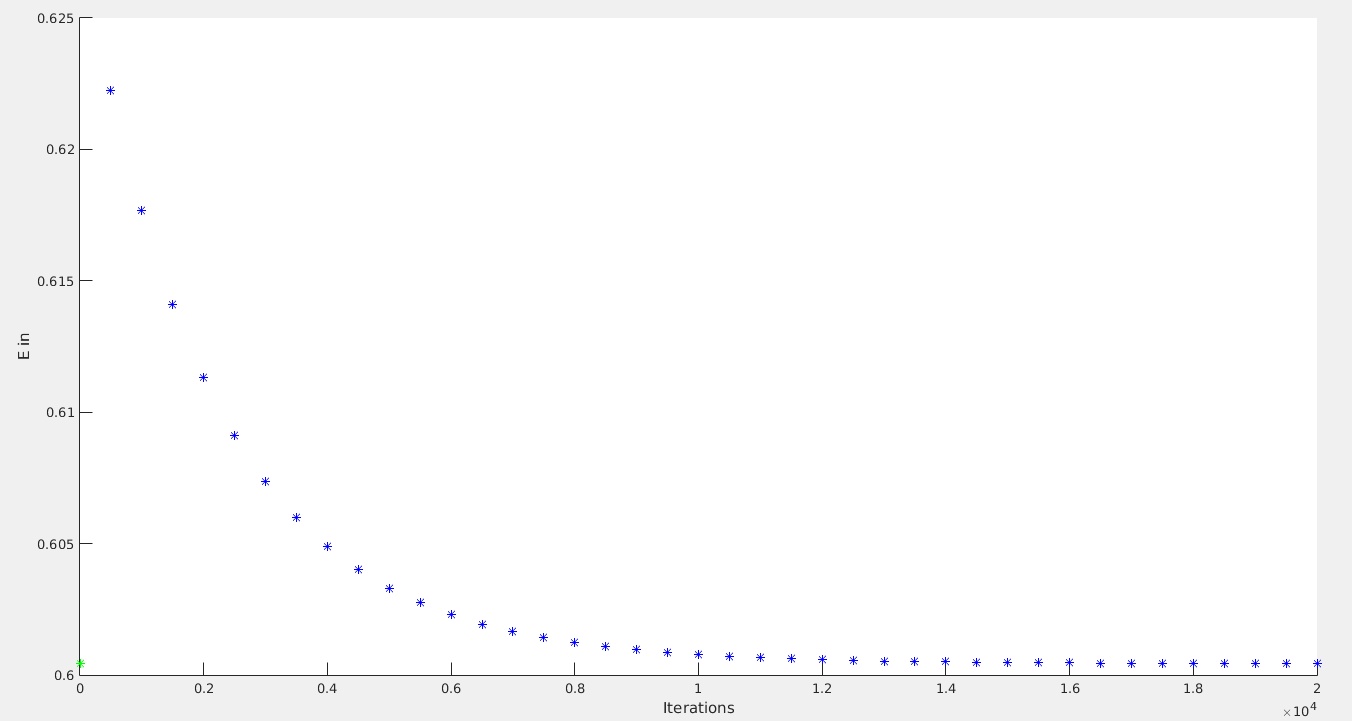
\includegraphics[scale=0.33]{fig3.png}
\end{center}
\caption{$E_{in}$ as a function of iterations}
\end{figure}


\subsection*{(8)}
We can use the calculation from (2). Changing the vector to the one we found in (6) gives us the probability $0.4886$.

\newpage
\section*{Question 3}
\subsection*{(1)}
From equation (2.1) in [LFD] we have that
\begin{align*}
E_{out}(g)\leq E_{in}(g)+\sqrt{\frac{1}{2N}\ln\frac{2M}{\delta}}
\end{align*}
The generalization bounds for predicting $\mathcal{H}_0$ where the upper bounds for $E_{out}$ holds with probability $1-\frac{\delta}{2}$ will be (number of hypotheses $M$ is $2$).
\begin{align*}
E_{out}(g)&\leq E_{in}(g)+\sqrt{\frac{1}{2N}\ln\frac{2\cdot 2}{\frac{\delta}{2}}} \\
&= E_{in}(g)+\sqrt{\frac{\ln\frac{8}{\delta}}{2N}}
\end{align*}
Similarly for $\mathcal{H}_8$, when the number of hypotheses are $2^8$ we get
\begin{align*}
E_{out}(g)&\leq E_{in}(g)+\sqrt{\frac{1}{2N}\ln\frac{2\cdot 2^8}{\frac{\delta}{2}}} \\
&= E_{in}(g)+\sqrt{\frac{\ln\frac{2^{10}}{\delta}}{2N}}
\end{align*}
Note that the bounds are a bit looser as they use the two-sided Hoeffding bound.

\end{document}